\documentclass{report}
\usepackage[utf8]{inputenc}
\usepackage[czech]{babel}
\usepackage{graphicx, import}
\usepackage{float}

\title{Deskriptor}
\author{Kateřina Kratochvílová}

% matematicke rovnice %
\usepackage{amsmath}
%odkazy%
\usepackage{hyperref}
%svg%
\usepackage{svg}

% #########
% # START #
% #########

\begin{document} 
% titulní stránka
%\maketitle
\begin{titlepage}
\begin{flushleft} 
{
\includegraphics[width=.5\textwidth]{./img/fav_logo.jpg}\\[3cm]}
\end{flushleft}
\begin{center}

{\Huge KIV/UIR - Semestrální práce}
\\[0.3cm]
\vspace{1.7cm}
{\Large Kateřina Kratochvílová} \\
\vspace{0.2cm}
{\normalsize dtwok8@students.zcu.cz}\\

{\large \today}
\end{center}
\end{titlepage}


% obsah
\tableofcontents
\thispagestyle{empty} %odstraneni cisla stranky z obsahu

% abstrakt
\begin{abstract}
abstrakt  
\end{abstract}


\chapter{Poem}
POEM (Patterns of Oriented Edge Magnitudes). Vstup algorimutmu se předpokládá šedotónový obrázek o rozměrech  $m \times n$.

\subsection{Výpočet gradientu a magnitudy}
Nejprve je potřeba vypočítat gradient. Gradient je obecně směr růstu. Výpočet může probíhat různými způsoby. Jednou z možností je použít masku, kterou aplikujeme na vstupní obrázek. Podle některých studii jsou nejlepší jednoduché masky jako je např. $[1, 0, -1]$ a $[1, 0, -1]^{\,t}$. Okraje obrázku se buď vypouštějí nebo se dají doplnit (opět existuje více způsobů).Výstupem jsou dva obrázky o rozměrech $m \times n$. \\
Na výstup se dá pohlíže také jako na vektor, kdy každý bod původního obrázku je reprezentován právě 2D vektorem. Analogicky pokud si vektory rozložíme na x a y složku dostaneme dva obrázky. Jeden, který reprezentuje obrázek po použití x-ového filtru, a druhý který reprezentuje obrázek po použití y-filtru. Přičemž použití y filtru by nám mělo zvýraznit hrany v y směru (svislé) a x zvýrazní hrany v x směru (vodorovné). \\
Magnituda je velikost směru růstu, lze si ji představit jako velikost směru růstu pro každý pixel (počítá se tedy pro každý pixel).  Z toho vyplývá, že ji můžeme spočítat jako velikost 2D vektorů, které jsme dostaly při výpočtu gradientu. Zjednodušeně magnituda představuje velikost vektoru gradientu. \\

Ukázka vstupního obrázku: 
\begin{displaymath} 
	\label{vstupni_matice} \begin{pmatrix}8 & 7 & 5 \\1 & 2 & 4 \\3 & 5 & 7 \end{pmatrix}
\end{displaymath}

Ukázka masky: 
\begin{align}
	\label{masky}
		maska(x) &= \begin{pmatrix}-1 & 1 \end{pmatrix} \\
		maska(y) &= \begin{pmatrix}-1 \\ 1 \end{pmatrix}
\end{align}

Ukázka gradientů:
\begin{align}
	\label{vystupni_gradienty}
		gradient(x) &= \begin{pmatrix}-1 & -2 & 0\\1 & 2 & 0 \\2 & 2 & 0 \end{pmatrix} \\
		gradient(y) &= \begin{pmatrix}-7 & -5 & -1 \\2 & 3 & 3 \\0 & 0 & 0 \end{pmatrix}
\end{align}

Gradient jako 2D vektory
\begin{align}
	\label{gradient_vektory} 
		\begin{pmatrix} 
			[-1 ; -7] & [-2 ; -5] & [0 ; -1] \\
			[1 ; 2] & [2 ; 3] & [0 ; 3] \\
			[2 ; 0] & [2 ; 0] & [0 ; 0] \\
		\end{pmatrix}		   
\end{align}

Vzoreček pro výpočet velikosti vektoru v rovině
\begin{align}
   \label{velikost_vektoru} |u| = \sqrt{u_1^2 + u_2^2}
\end{align}

\begin{figure}[htp]
	\centering
	\begin{minipage}[c]{150pt}
		\centering
		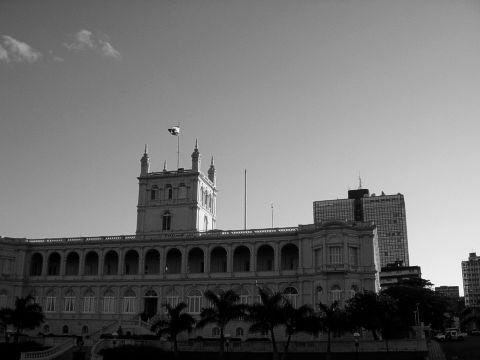
\includegraphics[width=150pt]{./img/vstupni_obraz.jpg}
		\caption{Vstupní obrázek}
	\end{minipage}
	\begin{minipage}[c]{150pt}
		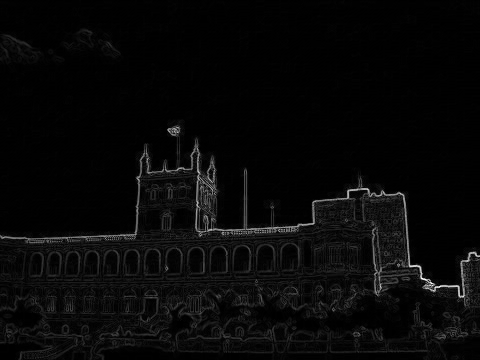
\includegraphics[width=150pt]{./img/magnitude.png}
		\caption{magnituda}
		\centering
	\end{minipage}
\end{figure}

\begin{figure}[htp]
	\centering
	\begin{minipage}[c]{150pt}
		\centering
		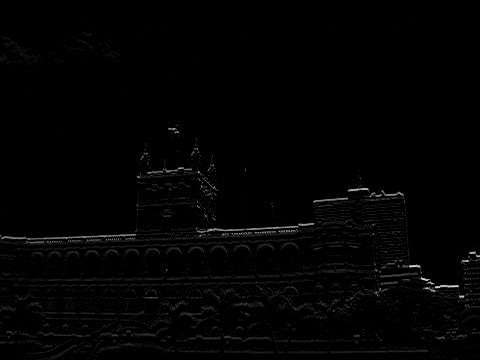
\includegraphics[width=150pt]{./img/gradientX.png}
		\caption{gradient x}
	\end{minipage}
	\begin{minipage}[c]{150pt}
		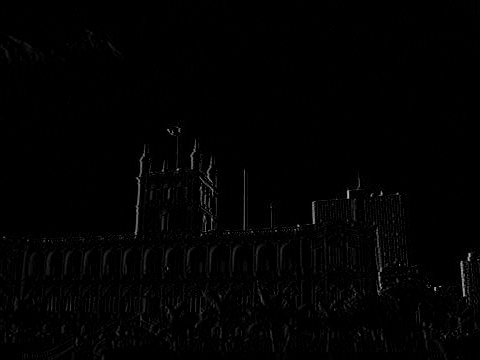
\includegraphics[width=150pt]{./img/gradientY.png}
		\caption{gradient y}
		\centering
	\end{minipage}
\end{figure}

\subsection{Diskretizace směru gradientu}
Pokud se na gradienty budeme koukat jako na 2D vektory můžeme určit nejen jejich velikost(magnitudu) ale i jejich směr. Je možné použít znaménkovou reprezentaci $0 - \pi$ nebo neznaménkovou reprezentaci $0 - 2\pi$.  V praxi si rovnoměrně rozdělíme kružnici na několik dílů (podle toho kolik chceme směrů). Označme si počet dílů $d$. Pro $d = 3$ znaménkovou reprezentaci to tedy bude $0 - \frac{2}{3}\pi$, $\frac{2}{3}\pi - \frac{4}{3}\pi$ a $\frac{3}{3}\pi - 2\pi$ 

\begin{figure}[ht]
	\centering
	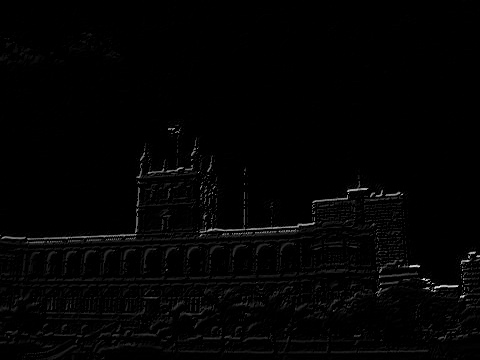
\includegraphics[width=150pt]{./img/directional0.jpg}
	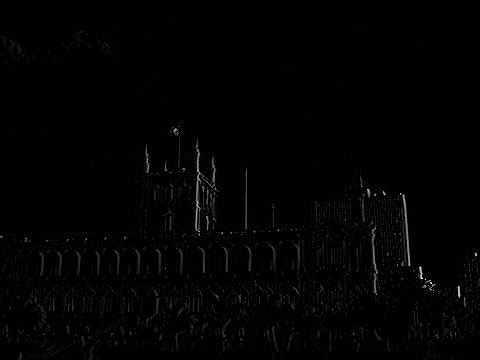
\includegraphics[width=150pt]{./img/directional1.jpg}
	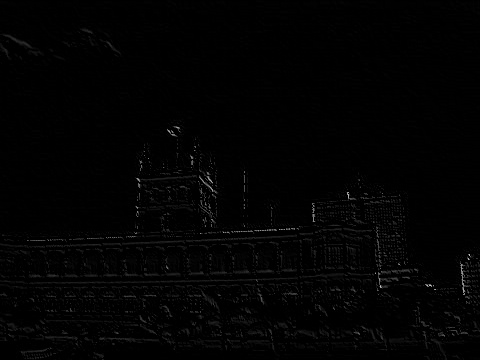
\includegraphics[width=150pt]{./img/directional2.jpg}
	\caption{Obrázky po diskretizaci. Každý obrázek představuje jeden směr.}
\end{figure}


\subsection{Výpočet lokálního histogramu orientace gradientů z okolí}
U každého směru projdeme jednotlivé pixely s jejich okolí a zprůměrujeme jejich hodnoty. Toto okolí se nazývá cell. Ukázka výpočtu u jednoho směru při velikosti cell 3. \\
 
Ukázka výpočtu u jednoho směru při velikosti cell 3
\begin{align}
	\label{aems}
		smer = \begin{pmatrix}0 & 0 & 0 & 0 \\ 0 & 0 & 0 & 0 \\0 & 0 & 0 & 0 \\ 0 & 3.6 & 3.6 & 3 \\ 0 & 2 & 2 & 0 \end{pmatrix}
		aems = \begin{pmatrix}0 & 0 \\ 0.8 & 1.1 \\ 1.2 & 1.5 \end{pmatrix}
\end{align}

Ukázka výpočtu pro jeden pixel při velikosti cell 3
\begin{align}
	\label{aems_detail}
		cell = \begin{pmatrix}0 & 0 & 0 \\ 0 & 3.6 & 3.6 \\ 0 & 2 & 2 \end{pmatrix}
		aems = \begin{pmatrix}0.8 \end{pmatrix}
\end{align}

\begin{figure}[H]
	\centering
	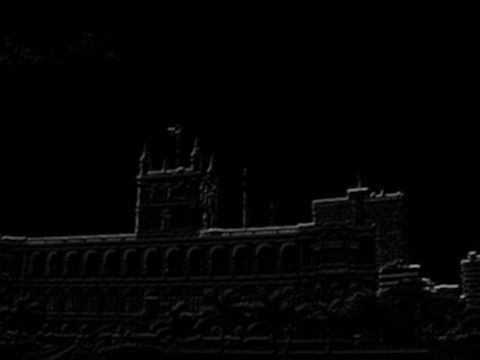
\includegraphics[width=150pt]{./img/aems0.png}
	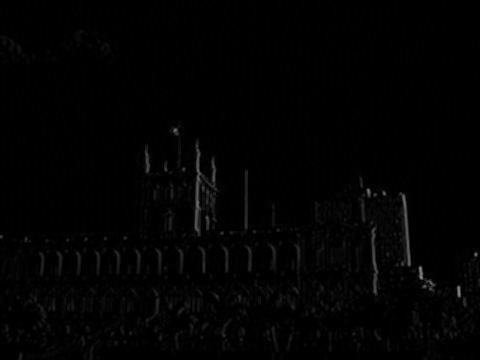
\includegraphics[width=150pt]{./img/aems1.png}
	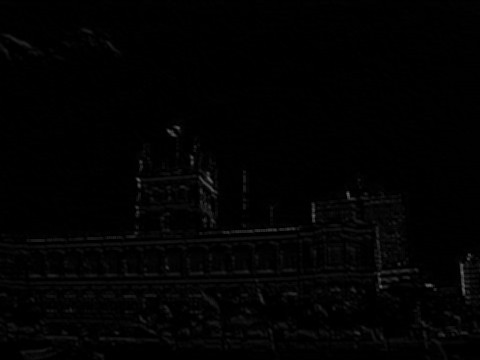
\includegraphics[width=150pt]{./img/aems2.png}
	\caption{Obrázky po výpočtu lokálních histogramů orientace gradientů . Každý obrázek představuje jeden směr.}
\end{figure}

\subsection{Zakódování příznaků pomocí LBP}
LBP operátor je aplikován na okolí každého pixelu o velikost $3 \times 3$. Oproti tomu POEM můžeme aplikovat na větší okolí. Toto okolí nazýváme block, zpravidla se jedná o kruhové okolí s poloměrem L/2. Pro stanovení intenzit okolních hodnot je možné použít bilineární interpolaci. Pokud bychom chtěli zvýšit stabilitu v téměř konstantní oblasti lze k centrálnímu pixelu přičítat malou konstantu $\tau$.

\begin{figure}[H]
		\centering
		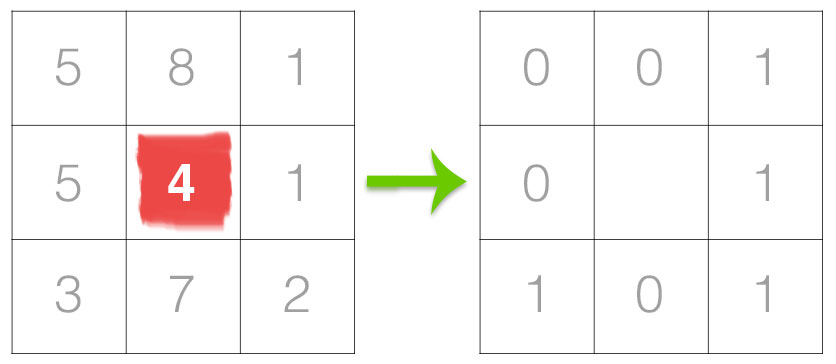
\includegraphics[width=200px]{./img/lbp_thresholding.jpg}
		\\[0.5cm]	
		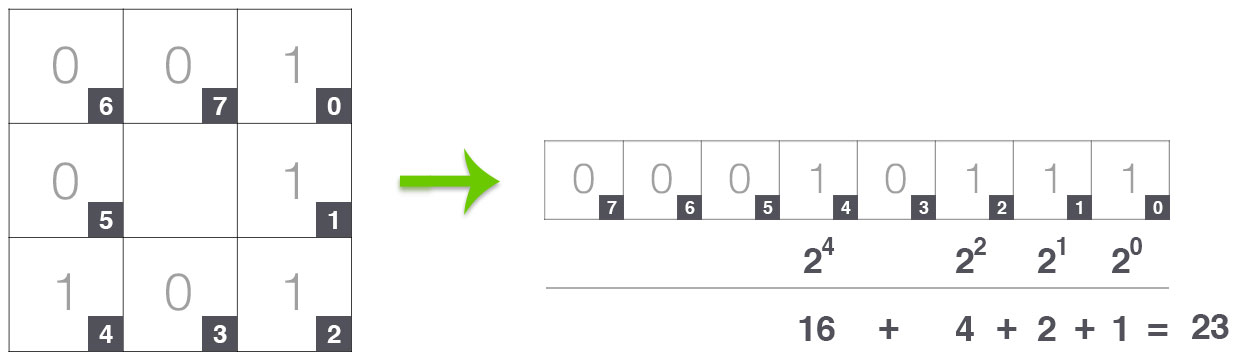
\includegraphics[width=350px]{./img/lbp_calculation.jpg}
		\\[0.5cm]
		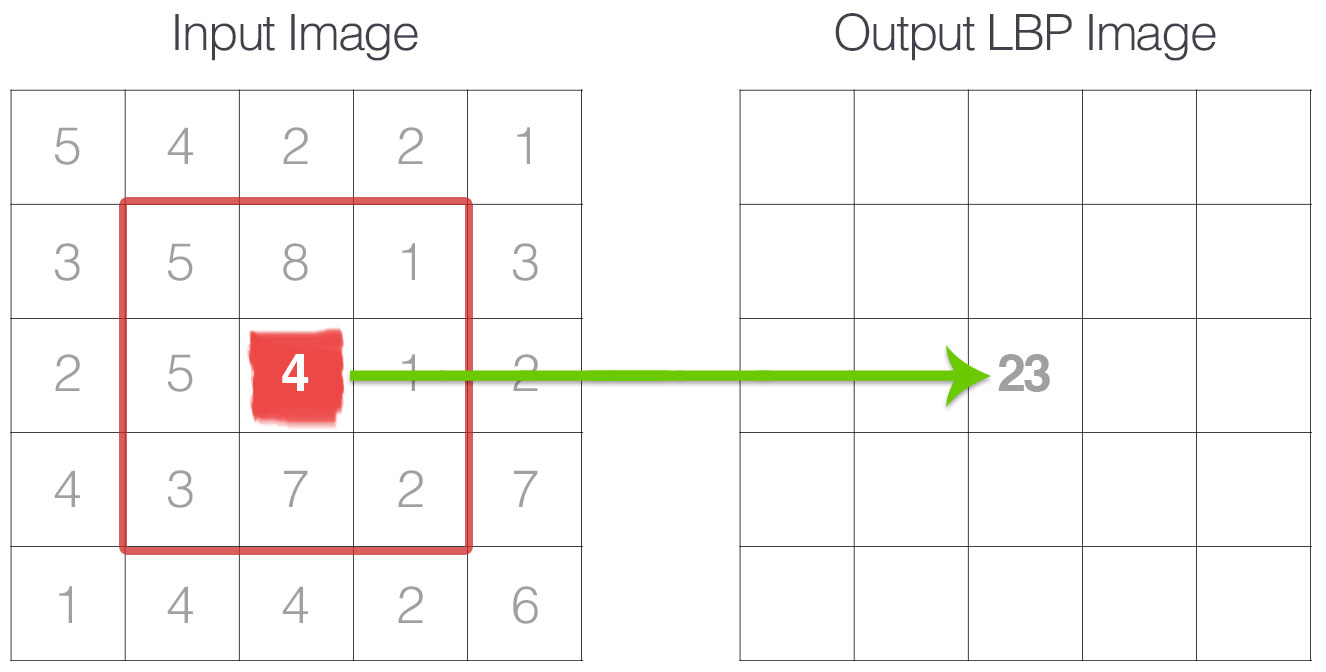
\includegraphics[width=253px]{./img/lbp_to_output.jpg}	
		\caption{Znázornění LBP}
\end{figure} 
 
\begin{figure}[H]
		\centering
		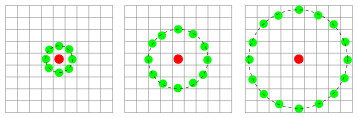
\includegraphics[width=253px]{./img/poem.png}	
		\caption{Znázornění POEM}
\end{figure}

\begin{figure}[H]
	\centering
	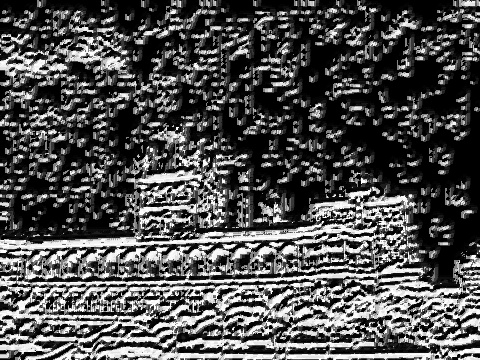
\includegraphics[width=150pt]{./img/lbp0.jpg}
	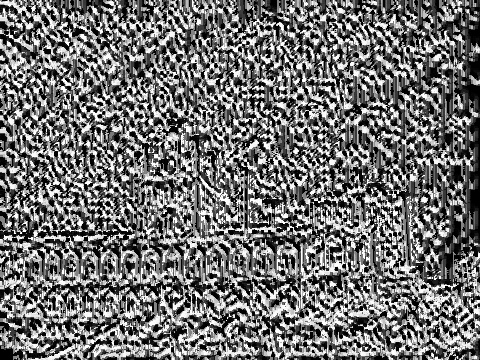
\includegraphics[width=150pt]{./img/lbp1.jpg}
	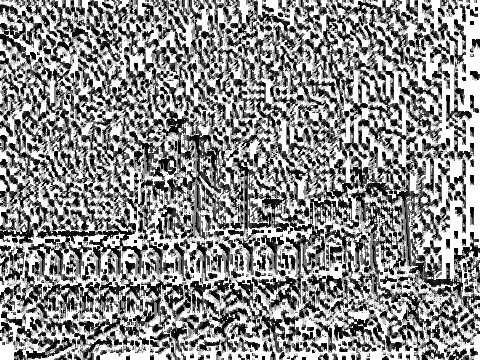
\includegraphics[width=150pt]{./img/lbp2.jpg}
	\caption{Obrázky po aplikaci POEM. Každý obrázek představuje jeden směr.}
\end{figure}

\begin{figure}[H]
	\centering
	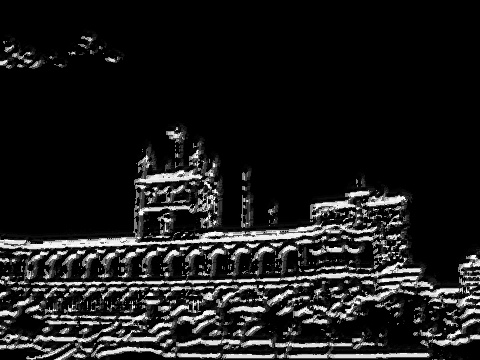
\includegraphics[width=150pt]{./img/lbp0_tau.jpg}
	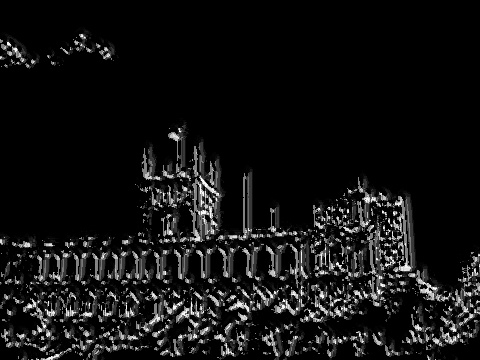
\includegraphics[width=150pt]{./img/lbp1_tau.jpg}
	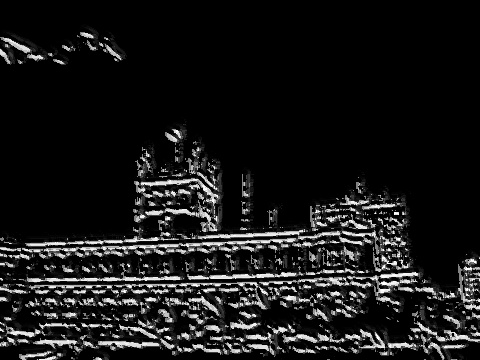
\includegraphics[width=150pt]{./img/lbp2_tau.jpg}
	\caption{Obrázky po aplikaci POEM při použití $\tau$. Každý obrázek představuje jeden směr.}
\end{figure} 

\subsection{Konstrukce globálního histogramu}
256 binu pro každý směr a zřetězí se.

\chapter{Barevný poem}
LBP i Gabor pracují s informací o intenzitě obrazu. Detekce hran. Obyčejné LBP problém s rotací.

kombinace textur a barevne informace
1. Vytvoření společného příznaku, 
například rozšíření LBP na všechny barvené kanály
informace o barvě a textuře se mohou oblivňovat protichůdně

2. Vyhodnotit a klasifikovat příznaky odděleně a pak výslednou klasifikaci nějak s pojit z několika částí 
	to je například JEC
	
	výhoda zachovává vlastnosti obou původních příznaků 
	výpočetně náročnější a jeho úspěšnost je přímo závislá na způsobu kombinace obou informací	
	
vutbrno 117319 10 stranka
\begin{figure}[h!]
    \centering    
    \def\svgwidth{\columnwidth}
	\import{img/}{image.pdf_tex}    
    %\input{image.pdf_tex}
    \caption{Your image caption}
    \label{fig:your image label}
\end{figure}


\begin{align}
   \label{velikost_vektoru_v_prostoru} |u| = \sqrt{u_1^2 + u_2^2 + u_3^2}
\end{align} 

\begin{align}
   \label{soucet_vektrou} \vec{u} + \vec{v} = (u_1 + v_1, u_2 + v_2, u_3 + v_3 )
\end{align} 
 

\chapter{Použité programové prostředky}
Program byl navržen na operační systému Linux. Jako programovací jazyk byl zvolen Python a to z důvodu jeho jednoduchého použití, což je na prototyp, jako je tento velice výhodné na časovou náročnost. Program využívá knihovnu OpenCV 3.1. 
  
\section{OpenCV}
OpenCV (Open source computer vision) je knihovna vydávána pod licencí BSD a je volně k dispozici jak pro akademické účely, tak pro komerční použití. Je vhodná pro použití v C++, C, Python a Javě. Podporuje operační systémy Windows, Linux, Mac OS, iOS a Android.
\\
Knihovna byla navrhnuta pro výpočetní efektivitu v oblasti počítačového vidění a zpracování obrazu se zaměřením na zpracování obrazu v reálném čase. Z důvodu optimalizace byla napsána v C/C++. 
\\
Knihovnu OpenCV je možné stáhnout na adrese: http://opencv.org/

\chapter{Závěr}
V teoretické části byly popsány nízkoúrovňové příznaky barva a textura. Byla rozebrána metoda JEC, která bude v bakalářské práci implementována. Seznamili jsme se s knihovnou OpenCV, prostudovali obrázk y apříložená metadata.

\chapter{Uživatelská dokumentace}
popsani jak vypada zdrojovej soubor kterej to zere, nejdriv cesta k souboru a pak jeho klicovy slova

\chapter{Zdroje}
\url{https://dspace5.zcu.cz/bitstream/11025/17883/1/A13N0110P.pdf} \\
\url{https://en.wikipedia.org/wiki/Local_binary_patterns} \\
\url{http://www.pyimagesearch.com/2015/12/07/local-binary-patterns-with-python-opencv/} \\


\end{document}